%--------------------------------------------------------------------------------------------------
%\subsection*{Average Drop}
%\begin{frame}[t]
%    \frametitle{Average Gain}
%    \framesubtitle{Motivation}
%    \small
%     Existing metrics for measuring interpretability (AD$\downarrow$, AI$\uparrow$), can be 
%     fooled.\\\pause
%     All pixels are salient \emph{but-one}:
%    \begin{columns}        
%        \column{.1\textwidth}
%        \column{.2\textwidth}
%            \begin{center}
%                {\footnotesize Input}\\
%                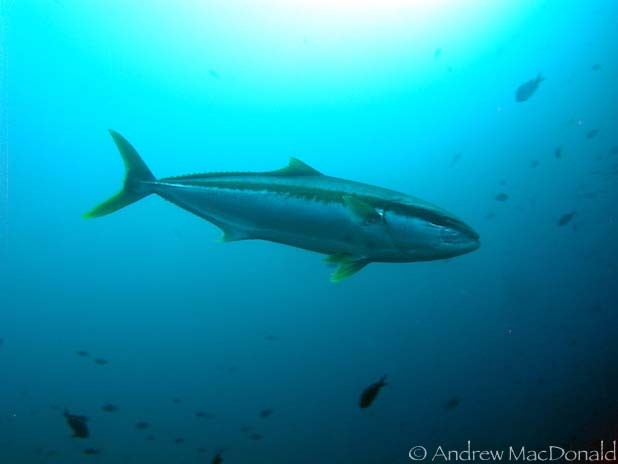
\includegraphics[width=\textwidth]{fig/opticam/common/img/ILSVRC2012_val_00000312.JPEG}
%                {\footnotesize $p_{389} = 0.874$}\\
%            \end{center}
%        \column{.2\textwidth}
%            \begin{center}
%                {\footnotesize Explanation}\\
%                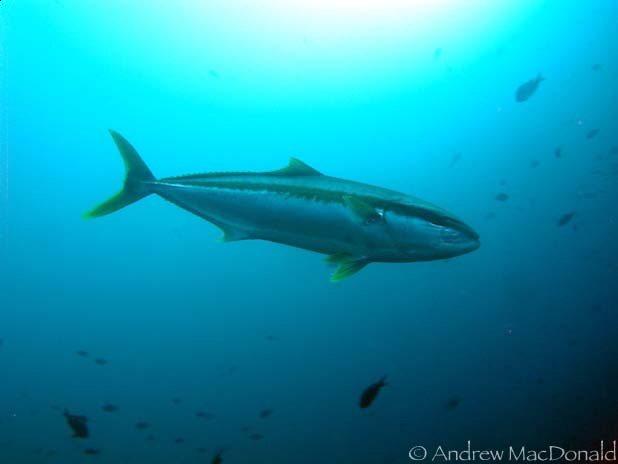
\includegraphics[width=\textwidth]{fig/opticam/common/img/exp.png}
%                {\footnotesize $o_{389} = 0.822$}
%            \end{center}    
%        \column{.5\textwidth}
%        {\footnotesize
%            \begin{itemize}
%                \item Drop = 5.95\%
%                \item Increase = 0\%
%            \end{itemize}
%        }
%    \end{columns}     
%    %\vspace{20pt}
%    %{\footnotesize Therefore, we don't drop much predictive power, \emph{but}, 
%    %we don't gain confidence in our prediciton.}
%    
%\end{frame}
%%--------------------------------------------------------------------------------------------------
%\begin{frame}[t]
%    \frametitle{Average Gain}
%    \framesubtitle{Definition}
%    \small
%    With the notation on  slide (\ref{slide:evaluation}):
%    \begin{center}
%        \begin{equation}
%            \mbox{AG(\%)} \defn \frac{1}{N}\sum_{i=1}^N\frac{[o_i^c-p_i^c]_+}{1-p_i^c} \cdot 100
%        \end{equation}
%    \end{center}
%    Measuring the increase in predictive power when masking an input.
%\end{frame}